\documentclass[border=3mm]{standalone}

\usepackage{tikz}

\begin{document}
	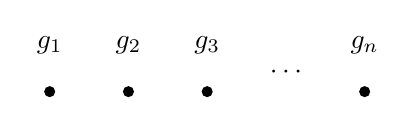
\begin{tikzpicture}
		\fill (0,0) circle (2pt) node[above,yshift=10pt] {$g_1$};
		\fill (1,0) circle (2pt) node[above,yshift=10pt] {$g_2$};
		\fill (2,0) circle (2pt) node[above,yshift=10pt] {$g_3$};
		\node at (3,0.25) {$\cdots$};
		\fill (4,0) circle (2pt) node[above,yshift=10pt] {$g_n$};
	\end{tikzpicture}
\end{document}